\documentclass[11pt]{book}
 
\newcommand{\reporttitle}{Coupling / Curtains}
\newcommand{\reportauthor}{CARIOU KOTLAREK}
\newcommand{\course}{Semester Paper}
\newcommand{\professor}{JACQUIER ; ACCIAIO}
% include file with configuration.
\input{../config/config_article} % various packages needed for maths etc.



\begin{document}


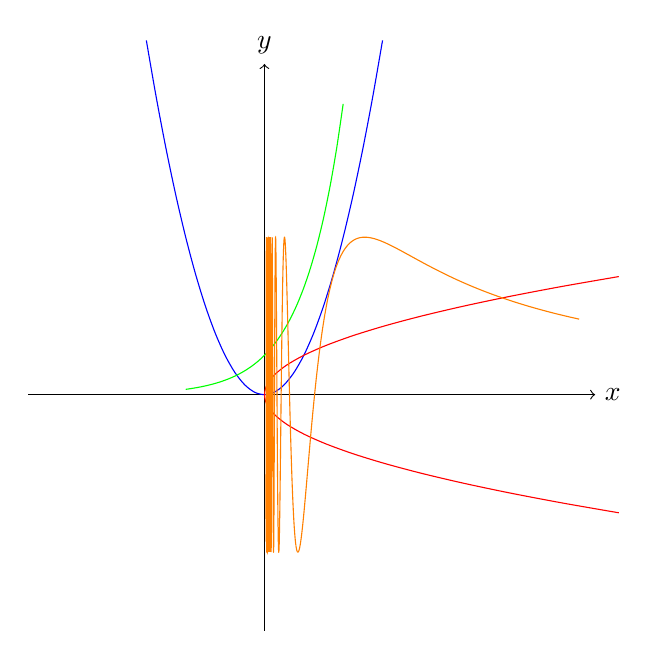
\begin{tikzpicture}
  \draw[->] (-3, 0) -- (4.2, 0) node[right] {$x$};
  \draw[->] (0, -3) -- (0, 4.2) node[above] {$y$};
  \draw[scale=0.5, domain=-3:3, smooth, variable=\x, blue] plot ({\x}, {\x*\x});
  \draw[scale=0.5, domain=-3:3, smooth, variable=\y, red]  plot ({\y*\y}, {\y});
  \draw[scale=0.5, domain=-2:2, smooth, variable=\z, green]  plot ({\z}, {exp(\z)});
  \draw[scale=2, domain=0.01:0.2, smooth, samples=1000, variable=\t, orange]  plot ({\t}, {sin(1/\t r)});
  \draw[scale=2, domain=0.2:2, smooth, samples=1000, variable=\w, orange]  plot ({\w}, {sin(1/\w r)});
  
\end{tikzpicture}




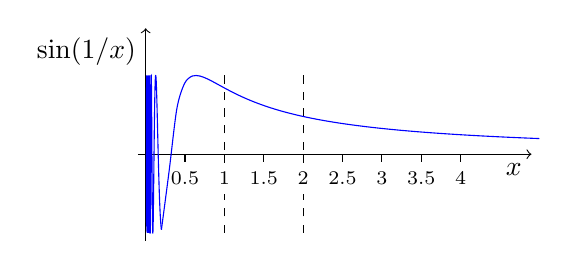
\begin{tikzpicture}
\draw[->]       (-0.1, 0) -- + (5,0) node[below left] {$x$};
\draw[->]       (0,-1.1) -- + (0,2.7) node[below left] {$\sin(1/x)$};
\draw[dashed]   (1,-1) -- + (0,2) (2,-1) -- + (0,2);
\foreach \i in {0.5, 1,...,4}
{
\draw (\i,0) -- + (0,-0.1) node[below,font=\scriptsize,fill=white] {\i};
}
\draw[blue,     samples=1000, domain=0.01:0.2] plot(\x, {sin(1/\x r)});
\draw[blue,smooth,samples=50, domain=0.2:5]    plot(\x, {sin(1/\x r)});
\end{tikzpicture}


\end{document}